\documentclass[1p]{elsarticle_modified}
%\bibliographystyle{elsarticle-num}

%\usepackage[colorlinks]{hyperref}
%\usepackage{abbrmath_seonhwa} %\Abb, \Ascr, \Acal ,\Abf, \Afrak
\usepackage{amsfonts}
\usepackage{amssymb}
\usepackage{amsmath}
\usepackage{amsthm}
\usepackage{scalefnt}
\usepackage{amsbsy}
\usepackage{kotex}
\usepackage{caption}
\usepackage{subfig}
\usepackage{color}
\usepackage{graphicx}
\usepackage{xcolor} %% white, black, red, green, blue, cyan, magenta, yellow
\usepackage{float}
\usepackage{setspace}
\usepackage{hyperref}

\usepackage{tikz}
\usetikzlibrary{arrows}

\usepackage{multirow}
\usepackage{array} % fixed length table
\usepackage{hhline}

%%%%%%%%%%%%%%%%%%%%%
\makeatletter
\renewcommand*\env@matrix[1][\arraystretch]{%
	\edef\arraystretch{#1}%
	\hskip -\arraycolsep
	\let\@ifnextchar\new@ifnextchar
	\array{*\c@MaxMatrixCols c}}
\makeatother %https://tex.stackexchange.com/questions/14071/how-can-i-increase-the-line-spacing-in-a-matrix
%%%%%%%%%%%%%%%

\usepackage[normalem]{ulem}

\newcommand{\msout}[1]{\ifmmode\text{\sout{\ensuremath{#1}}}\else\sout{#1}\fi}
%SOURCE: \msout is \stkout macro in https://tex.stackexchange.com/questions/20609/strikeout-in-math-mode

\newcommand{\cancel}[1]{
	\ifmmode
	{\color{red}\msout{#1}}
	\else
	{\color{red}\sout{#1}}
	\fi
}

\newcommand{\add}[1]{
	{\color{blue}\uwave{#1}}
}

\newcommand{\replace}[2]{
	\ifmmode
	{\color{red}\msout{#1}}{\color{blue}\uwave{#2}}
	\else
	{\color{red}\sout{#1}}{\color{blue}\uwave{#2}}
	\fi
}

\newcommand{\Sol}{\mathcal{S}} %segment
\newcommand{\D}{D} %diagram
\newcommand{\A}{\mathcal{A}} %arc


%%%%%%%%%%%%%%%%%%%%%%%%%%%%%5 test

\def\sl{\operatorname{\textup{SL}}(2,\Cbb)}
\def\psl{\operatorname{\textup{PSL}}(2,\Cbb)}
\def\quan{\mkern 1mu \triangleright \mkern 1mu}

\theoremstyle{definition}
\newtheorem{thm}{Theorem}[section]
\newtheorem{prop}[thm]{Proposition}
\newtheorem{lem}[thm]{Lemma}
\newtheorem{ques}[thm]{Question}
\newtheorem{cor}[thm]{Corollary}
\newtheorem{defn}[thm]{Definition}
\newtheorem{exam}[thm]{Example}
\newtheorem{rmk}[thm]{Remark}
\newtheorem{alg}[thm]{Algorithm}

\newcommand{\I}{\sqrt{-1}}
\begin{document}

%\begin{frontmatter}
%
%\title{Boundary parabolic representations of knots up to 8 crossings}
%
%%% Group authors per affiliation:
%\author{Yunhi Cho} 
%\address{Department of Mathematics, University of Seoul, Seoul, Korea}
%\ead{yhcho@uos.ac.kr}
%
%
%\author{Seonhwa Kim} %\fnref{s_kim}}
%\address{Center for Geometry and Physics, Institute for Basic Science, Pohang, 37673, Korea}
%\ead{ryeona17@ibs.re.kr}
%
%\author{Hyuk Kim}
%\address{Department of Mathematical Sciences, Seoul National University, Seoul 08826, Korea}
%\ead{hyukkim@snu.ac.kr}
%
%\author{Seokbeom Yoon}
%\address{Department of Mathematical Sciences, Seoul National University, Seoul, 08826,  Korea}
%\ead{sbyoon15@snu.ac.kr}
%
%\begin{abstract}
%We find all boundary parabolic representation of knots up to 8 crossings.
%
%\end{abstract}
%\begin{keyword}
%    \MSC[2010] 57M25 
%\end{keyword}
%
%\end{frontmatter}

%\linenumbers
%\tableofcontents
%
\newcommand\colored[1]{\textcolor{white}{\rule[-0.35ex]{0.8em}{1.4ex}}\kern-0.8em\color{red} #1}%
%\newcommand\colored[1]{\textcolor{white}{ #1}\kern-2.17ex	\textcolor{white}{ #1}\kern-1.81ex	\textcolor{white}{ #1}\kern-2.15ex\color{red}#1	}

{\Large $\underline{12n_{0252}~(K12n_{0252})}$}

\setlength{\tabcolsep}{10pt}
\renewcommand{\arraystretch}{1.6}
\vspace{1cm}\begin{tabular}{m{100pt}>{\centering\arraybackslash}m{274pt}}
\multirow{5}{120pt}{
	\centering
	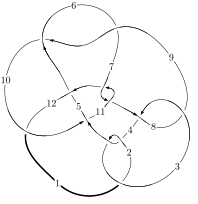
\includegraphics[width=112pt]{../../../GIT/diagram.site/Diagrams/png/2341_12n_0252.png}\\
\ \ \ A knot diagram\footnotemark}&
\allowdisplaybreaks
\textbf{Linearized knot diagam} \\
\cline{2-2}
 &
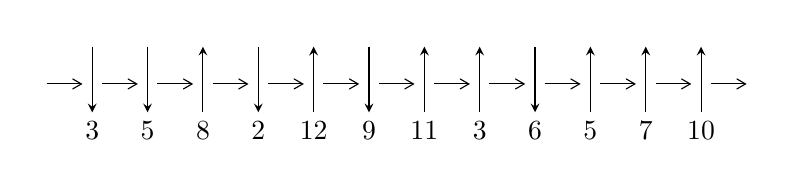
\begin{tikzpicture}[x=20pt, y=17pt]
	% nodes
	\node (C0) at (0, 0) {};
	\node (C1) at (1, 0) {};
	\node (C1U) at (1, +1) {};
	\node (C1D) at (1, -1) {3};

	\node (C2) at (2, 0) {};
	\node (C2U) at (2, +1) {};
	\node (C2D) at (2, -1) {5};

	\node (C3) at (3, 0) {};
	\node (C3U) at (3, +1) {};
	\node (C3D) at (3, -1) {8};

	\node (C4) at (4, 0) {};
	\node (C4U) at (4, +1) {};
	\node (C4D) at (4, -1) {2};

	\node (C5) at (5, 0) {};
	\node (C5U) at (5, +1) {};
	\node (C5D) at (5, -1) {12};

	\node (C6) at (6, 0) {};
	\node (C6U) at (6, +1) {};
	\node (C6D) at (6, -1) {9};

	\node (C7) at (7, 0) {};
	\node (C7U) at (7, +1) {};
	\node (C7D) at (7, -1) {11};

	\node (C8) at (8, 0) {};
	\node (C8U) at (8, +1) {};
	\node (C8D) at (8, -1) {3};

	\node (C9) at (9, 0) {};
	\node (C9U) at (9, +1) {};
	\node (C9D) at (9, -1) {6};

	\node (C10) at (10, 0) {};
	\node (C10U) at (10, +1) {};
	\node (C10D) at (10, -1) {5};

	\node (C11) at (11, 0) {};
	\node (C11U) at (11, +1) {};
	\node (C11D) at (11, -1) {7};

	\node (C12) at (12, 0) {};
	\node (C12U) at (12, +1) {};
	\node (C12D) at (12, -1) {10};
	\node (C13) at (13, 0) {};

	% arrows
	\draw[->,>={angle 60}]
	(C0) edge (C1) (C1) edge (C2) (C2) edge (C3) (C3) edge (C4) (C4) edge (C5) (C5) edge (C6) (C6) edge (C7) (C7) edge (C8) (C8) edge (C9) (C9) edge (C10) (C10) edge (C11) (C11) edge (C12) (C12) edge (C13) ;	\draw[->,>=stealth]
	(C1U) edge (C1D) (C2U) edge (C2D) (C3D) edge (C3U) (C4U) edge (C4D) (C5D) edge (C5U) (C6U) edge (C6D) (C7D) edge (C7U) (C8D) edge (C8U) (C9U) edge (C9D) (C10D) edge (C10U) (C11D) edge (C11U) (C12D) edge (C12U) ;
	\end{tikzpicture} \\
\hhline{~~} \\& 
\textbf{Solving Sequence} \\ \cline{2-2} 
 &
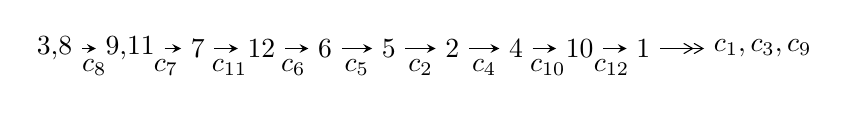
\begin{tikzpicture}[x=23pt, y=7pt]
	% node
	\node (A0) at (-1/8, 0) {3,8};
	\node (A1) at (17/16, 0) {9,11};
	\node (A2) at (17/8, 0) {7};
	\node (A3) at (25/8, 0) {12};
	\node (A4) at (33/8, 0) {6};
	\node (A5) at (41/8, 0) {5};
	\node (A6) at (49/8, 0) {2};
	\node (A7) at (57/8, 0) {4};
	\node (A8) at (65/8, 0) {10};
	\node (A9) at (73/8, 0) {1};
	\node (C1) at (1/2, -1) {$c_{8}$};
	\node (C2) at (13/8, -1) {$c_{7}$};
	\node (C3) at (21/8, -1) {$c_{11}$};
	\node (C4) at (29/8, -1) {$c_{6}$};
	\node (C5) at (37/8, -1) {$c_{5}$};
	\node (C6) at (45/8, -1) {$c_{2}$};
	\node (C7) at (53/8, -1) {$c_{4}$};
	\node (C8) at (61/8, -1) {$c_{10}$};
	\node (C9) at (69/8, -1) {$c_{12}$};
	\node (A10) at (11, 0) {$c_{1},c_{3},c_{9}$};

	% edge
	\draw[->,>=stealth]	
	(A0) edge (A1) (A1) edge (A2) (A2) edge (A3) (A3) edge (A4) (A4) edge (A5) (A5) edge (A6) (A6) edge (A7) (A7) edge (A8) (A8) edge (A9) ;
	\draw[->>,>={angle 60}]	
	(A9) edge (A10);
\end{tikzpicture} \\ 

\end{tabular} \\

\footnotetext{
The image of knot diagram is generated by the software ``\textbf{Draw programme}" developed by Andrew Bartholomew(\url{http://www.layer8.co.uk/maths/draw/index.htm\#Running-draw}), where we modified some parts for our purpose(\url{https://github.com/CATsTAILs/LinksPainter}).
}\phantom \\ \newline 
\centering \textbf{Ideals for irreducible components\footnotemark of $X_{\text{par}}$} 
 
\begin{align*}
I^u_{1}&=\langle 
1.74295\times10^{297} u^{66}+2.18772\times10^{297} u^{65}+\cdots+1.47028\times10^{301} b-2.20085\times10^{301},\\
\phantom{I^u_{1}}&\phantom{= \langle  }6.14451\times10^{299} u^{66}+6.93121\times10^{299} u^{65}+\cdots+1.44088\times10^{303} a-3.76767\times10^{303},\\
\phantom{I^u_{1}}&\phantom{= \langle  }u^{67}+u^{66}+\cdots+43008 u-25088\rangle \\
I^u_{2}&=\langle 
94430 u^{13}-176465 u^{12}+\cdots+3057583 b-933114,\\
\phantom{I^u_{2}}&\phantom{= \langle  }14500551 u^{13}-6850118 u^{12}+\cdots+3057583 a+662027,\\
\phantom{I^u_{2}}&\phantom{= \langle  }u^{14}+3 u^{12}+3 u^{11}-5 u^{10}-4 u^9-11 u^8-8 u^7+12 u^6-8 u^5+20 u^4+6 u^2+u+1\rangle \\
\\
I^v_{1}&=\langle 
a,\;82026 v^8-2033115 v^7+\cdots+764761 b-1552510,\\
\phantom{I^v_{1}}&\phantom{= \langle  }7 v^9-3 v^8+2 v^7+14 v^6-23 v^5-33 v^4- v^3+8 v^2+v-1\rangle \\
\end{align*}
\raggedright * 3 irreducible components of $\dim_{\mathbb{C}}=0$, with total 90 representations.\\
\footnotetext{All coefficients of polynomials are rational numbers. But the coefficients are sometimes approximated in decimal forms when there is not enough margin.}
\newpage
\renewcommand{\arraystretch}{1}
\centering \section*{I. $I^u_{1}= \langle 1.74\times10^{297} u^{66}+2.19\times10^{297} u^{65}+\cdots+1.47\times10^{301} b-2.20\times10^{301},\;6.14\times10^{299} u^{66}+6.93\times10^{299} u^{65}+\cdots+1.44\times10^{303} a-3.77\times10^{303},\;u^{67}+u^{66}+\cdots+43008 u-25088 \rangle$}
\flushleft \textbf{(i) Arc colorings}\\
\begin{tabular}{m{7pt} m{180pt} m{7pt} m{180pt} }
\flushright $a_{3}=$&$\begin{pmatrix}0\\u\end{pmatrix}$ \\
\flushright $a_{8}=$&$\begin{pmatrix}1\\0\end{pmatrix}$ \\
\flushright $a_{9}=$&$\begin{pmatrix}1\\- u^2\end{pmatrix}$ \\
\flushright $a_{11}=$&$\begin{pmatrix}-0.000426443 u^{66}-0.000481041 u^{65}+\cdots+23.8714 u+2.61485\\-0.000118545 u^{66}-0.000148796 u^{65}+\cdots+1.19020 u+1.49689\end{pmatrix}$ \\
\flushright $a_{7}=$&$\begin{pmatrix}-0.000247541 u^{66}-0.000147912 u^{65}+\cdots+24.8866 u-6.57361\\-0.0000205091 u^{66}+0.0000421361 u^{65}+\cdots+10.5559 u-4.84697\end{pmatrix}$ \\
\flushright $a_{12}=$&$\begin{pmatrix}0.000153563 u^{66}+0.000170524 u^{65}+\cdots-8.86925 u-0.350734\\0.0000954123 u^{66}+0.0000873267 u^{65}+\cdots-8.78651 u+0.999057\end{pmatrix}$ \\
\flushright $a_{6}=$&$\begin{pmatrix}-0.000167486 u^{66}-0.0000324937 u^{65}+\cdots+24.9473 u-8.92109\\7.23133\times10^{-6} u^{66}+0.0000863901 u^{65}+\cdots+10.0683 u-5.73416\end{pmatrix}$ \\
\flushright $a_{5}=$&$\begin{pmatrix}-0.0000140055 u^{66}-0.0000216075 u^{65}+\cdots+1.31456 u+0.105113\\-7.78737\times10^{-6} u^{66}-0.0000120618 u^{65}+\cdots+0.998848 u-0.412656\end{pmatrix}$ \\
\flushright $a_{2}=$&$\begin{pmatrix}6.21813\times10^{-6} u^{66}+9.54570\times10^{-6} u^{65}+\cdots-0.315708 u-0.517768\\-7.78737\times10^{-6} u^{66}-0.0000120618 u^{65}+\cdots+0.998848 u-0.412656\end{pmatrix}$ \\
\flushright $a_{4}=$&$\begin{pmatrix}u\\u\end{pmatrix}$ \\
\flushright $a_{10}=$&$\begin{pmatrix}-0.000359878 u^{66}-0.000389095 u^{65}+\cdots+22.6042 u+1.99943\\-0.0000816759 u^{66}-0.0000928007 u^{65}+\cdots+1.70659 u+1.44097\end{pmatrix}$ \\
\flushright $a_{1}=$&$\begin{pmatrix}-6.21813\times10^{-6} u^{66}-9.54570\times10^{-6} u^{65}+\cdots+0.315708 u+0.517768\\4.29248\times10^{-6} u^{66}+5.85448\times10^{-6} u^{65}+\cdots-0.985959 u+0.496138\end{pmatrix}$\\&\end{tabular}
\flushleft \textbf{(ii) Obstruction class $= -1$}\\~\\
\flushleft \textbf{(iii) Cusp Shapes $= 0.000336583 u^{66}+0.000559671 u^{65}+\cdots-0.882700 u-3.59196$}\\~\\
\newpage\renewcommand{\arraystretch}{1}
\flushleft \textbf{(iv) u-Polynomials at the component}\newline \\
\begin{tabular}{m{50pt}|m{274pt}}
Crossings & \hspace{64pt}u-Polynomials at each crossing \\
\hline $$\begin{aligned}c_{1}\end{aligned}$$&$\begin{aligned}
&u^{67}+78 u^{66}+\cdots+171200 u+2401
\end{aligned}$\\
\hline $$\begin{aligned}c_{2},c_{4}\end{aligned}$$&$\begin{aligned}
&u^{67}-16 u^{66}+\cdots+120 u-49
\end{aligned}$\\
\hline $$\begin{aligned}c_{3},c_{8}\end{aligned}$$&$\begin{aligned}
&u^{67}+u^{66}+\cdots+43008 u-25088
\end{aligned}$\\
\hline $$\begin{aligned}c_{5}\end{aligned}$$&$\begin{aligned}
&u^{67}+4 u^{66}+\cdots-2 u-1
\end{aligned}$\\
\hline $$\begin{aligned}c_{6},c_{9}\end{aligned}$$&$\begin{aligned}
&u^{67}-3 u^{66}+\cdots+781 u-209
\end{aligned}$\\
\hline $$\begin{aligned}c_{7},c_{11}\end{aligned}$$&$\begin{aligned}
&u^{67}-2 u^{66}+\cdots+3200 u-773
\end{aligned}$\\
\hline $$\begin{aligned}c_{10}\end{aligned}$$&$\begin{aligned}
&u^{67}+u^{66}+\cdots+566773 u-256243
\end{aligned}$\\
\hline $$\begin{aligned}c_{12}\end{aligned}$$&$\begin{aligned}
&u^{67}+12 u^{66}+\cdots-77902 u-10969
\end{aligned}$\\
\hline
\end{tabular}\\~\\
\newpage\renewcommand{\arraystretch}{1}
\flushleft \textbf{(v) Riley Polynomials at the component}\newline \\
\begin{tabular}{m{50pt}|m{274pt}}
Crossings & \hspace{64pt}Riley Polynomials at each crossing \\
\hline $$\begin{aligned}c_{1}\end{aligned}$$&$\begin{aligned}
&y^{67}-162 y^{66}+\cdots+5062883876 y-5764801
\end{aligned}$\\
\hline $$\begin{aligned}c_{2},c_{4}\end{aligned}$$&$\begin{aligned}
&y^{67}-78 y^{66}+\cdots+171200 y-2401
\end{aligned}$\\
\hline $$\begin{aligned}c_{3},c_{8}\end{aligned}$$&$\begin{aligned}
&y^{67}+63 y^{66}+\cdots-2491940864 y-629407744
\end{aligned}$\\
\hline $$\begin{aligned}c_{5}\end{aligned}$$&$\begin{aligned}
&y^{67}-10 y^{66}+\cdots-44 y-1
\end{aligned}$\\
\hline $$\begin{aligned}c_{6},c_{9}\end{aligned}$$&$\begin{aligned}
&y^{67}+33 y^{66}+\cdots-240251 y-43681
\end{aligned}$\\
\hline $$\begin{aligned}c_{7},c_{11}\end{aligned}$$&$\begin{aligned}
&y^{67}+62 y^{66}+\cdots-18480042 y-597529
\end{aligned}$\\
\hline $$\begin{aligned}c_{10}\end{aligned}$$&$\begin{aligned}
&y^{67}+43 y^{66}+\cdots+161121782381 y-65660475049
\end{aligned}$\\
\hline $$\begin{aligned}c_{12}\end{aligned}$$&$\begin{aligned}
&y^{67}+16 y^{66}+\cdots-1081596550 y-120318961
\end{aligned}$\\
\hline
\end{tabular}\\~\\
\newpage\flushleft \textbf{(vi) Complex Volumes and Cusp Shapes}
$$\begin{array}{c|c|c}  
\text{Solutions to }I^u_{1}& \I (\text{vol} + \sqrt{-1}CS) & \text{Cusp shape}\\
 \hline 
\begin{aligned}
u &= -0.972237 + 0.280854 I \\
a &= \phantom{-}0.153697 + 0.835171 I \\
b &= \phantom{-}0.437985 + 0.887119 I\end{aligned}
 & \phantom{-}3.39425 - 2.09087 I & \phantom{-}8.43522 + 3.94985 I \\ \hline\begin{aligned}
u &= -0.972237 - 0.280854 I \\
a &= \phantom{-}0.153697 - 0.835171 I \\
b &= \phantom{-}0.437985 - 0.887119 I\end{aligned}
 & \phantom{-}3.39425 + 2.09087 I & \phantom{-}8.43522 - 3.94985 I \\ \hline\begin{aligned}
u &= -0.111044 + 1.030770 I \\
a &= -0.447368 - 0.244256 I \\
b &= -1.094900 + 0.275542 I\end{aligned}
 & \phantom{-}0.89656 - 5.19617 I & \phantom{-}2.00000 + 8.56770 I \\ \hline\begin{aligned}
u &= -0.111044 - 1.030770 I \\
a &= -0.447368 + 0.244256 I \\
b &= -1.094900 - 0.275542 I\end{aligned}
 & \phantom{-}0.89656 + 5.19617 I & \phantom{-}2.00000 - 8.56770 I \\ \hline\begin{aligned}
u &= \phantom{-}0.502448 + 0.771343 I \\
a &= \phantom{-}0.544773 + 0.292063 I \\
b &= \phantom{-}0.060296 - 0.570771 I\end{aligned}
 & \phantom{-}0.42745 + 2.04731 I & \phantom{-}1.79133 - 2.30943 I \\ \hline\begin{aligned}
u &= \phantom{-}0.502448 - 0.771343 I \\
a &= \phantom{-}0.544773 - 0.292063 I \\
b &= \phantom{-}0.060296 + 0.570771 I\end{aligned}
 & \phantom{-}0.42745 - 2.04731 I & \phantom{-}1.79133 + 2.30943 I \\ \hline\begin{aligned}
u &= -0.163401 + 0.813880 I \\
a &= \phantom{-}0.496846 + 0.323676 I \\
b &= \phantom{-}0.477457 + 0.309386 I\end{aligned}
 & -1.58473 + 1.12240 I & -2.95098 - 3.87144 I \\ \hline\begin{aligned}
u &= -0.163401 - 0.813880 I \\
a &= \phantom{-}0.496846 - 0.323676 I \\
b &= \phantom{-}0.477457 - 0.309386 I\end{aligned}
 & -1.58473 - 1.12240 I & -2.95098 + 3.87144 I \\ \hline\begin{aligned}
u &= -0.687972 + 0.429990 I \\
a &= \phantom{-}1.266640 - 0.347433 I \\
b &= -0.201497 + 0.581210 I\end{aligned}
 & -2.34582 + 0.79184 I & -1.70277 + 1.36728 I \\ \hline\begin{aligned}
u &= -0.687972 - 0.429990 I \\
a &= \phantom{-}1.266640 + 0.347433 I \\
b &= -0.201497 - 0.581210 I\end{aligned}
 & -2.34582 - 0.79184 I & -1.70277 - 1.36728 I\\
 \hline 
 \end{array}$$\newpage$$\begin{array}{c|c|c}  
\text{Solutions to }I^u_{1}& \I (\text{vol} + \sqrt{-1}CS) & \text{Cusp shape}\\
 \hline 
\begin{aligned}
u &= -0.423056 + 1.121960 I \\
a &= \phantom{-}0.352233 - 0.211840 I \\
b &= -0.121837 + 0.470824 I\end{aligned}
 & -4.49098 - 4.90499 I & \phantom{-0.000000 } 0 \\ \hline\begin{aligned}
u &= -0.423056 - 1.121960 I \\
a &= \phantom{-}0.352233 + 0.211840 I \\
b &= -0.121837 - 0.470824 I\end{aligned}
 & -4.49098 + 4.90499 I & \phantom{-0.000000 } 0 \\ \hline\begin{aligned}
u &= -0.683441 + 0.994440 I \\
a &= \phantom{-}1.027540 + 0.560982 I \\
b &= \phantom{-}0.204096 + 1.284980 I\end{aligned}
 & -2.72054 + 1.47592 I & \phantom{-0.000000 } 0 \\ \hline\begin{aligned}
u &= -0.683441 - 0.994440 I \\
a &= \phantom{-}1.027540 - 0.560982 I \\
b &= \phantom{-}0.204096 - 1.284980 I\end{aligned}
 & -2.72054 - 1.47592 I & \phantom{-0.000000 } 0 \\ \hline\begin{aligned}
u &= \phantom{-}0.412259 + 0.668041 I \\
a &= -1.50421 + 0.97445 I \\
b &= -0.172196 - 0.202734 I\end{aligned}
 & \phantom{-}0.01538 + 1.90218 I & \phantom{-}1.03416 - 1.99152 I \\ \hline\begin{aligned}
u &= \phantom{-}0.412259 - 0.668041 I \\
a &= -1.50421 - 0.97445 I \\
b &= -0.172196 + 0.202734 I\end{aligned}
 & \phantom{-}0.01538 - 1.90218 I & \phantom{-}1.03416 + 1.99152 I \\ \hline\begin{aligned}
u &= -0.734728 + 0.191087 I \\
a &= \phantom{-}0.112393 - 1.136120 I \\
b &= \phantom{-}0.561939 - 0.465578 I\end{aligned}
 & \phantom{-}3.56178 + 1.95197 I & \phantom{-}9.44446 - 1.83557 I \\ \hline\begin{aligned}
u &= -0.734728 - 0.191087 I \\
a &= \phantom{-}0.112393 + 1.136120 I \\
b &= \phantom{-}0.561939 + 0.465578 I\end{aligned}
 & \phantom{-}3.56178 - 1.95197 I & \phantom{-}9.44446 + 1.83557 I \\ \hline\begin{aligned}
u &= \phantom{-}0.705362 + 0.112303 I \\
a &= -3.77447 - 2.00026 I \\
b &= \phantom{-}0.813283 + 0.575619 I\end{aligned}
 & -0.78374 + 3.24647 I & \phantom{-}3.36554 - 8.05825 I \\ \hline\begin{aligned}
u &= \phantom{-}0.705362 - 0.112303 I \\
a &= -3.77447 + 2.00026 I \\
b &= \phantom{-}0.813283 - 0.575619 I\end{aligned}
 & -0.78374 - 3.24647 I & \phantom{-}3.36554 + 8.05825 I\\
 \hline 
 \end{array}$$\newpage$$\begin{array}{c|c|c}  
\text{Solutions to }I^u_{1}& \I (\text{vol} + \sqrt{-1}CS) & \text{Cusp shape}\\
 \hline 
\begin{aligned}
u &= \phantom{-}0.489130 + 0.496557 I \\
a &= \phantom{-}0.706509 + 0.025107 I \\
b &= -0.474253 - 0.853751 I\end{aligned}
 & \phantom{-}0.85096 + 2.02536 I & \phantom{-}5.69785 - 3.31418 I \\ \hline\begin{aligned}
u &= \phantom{-}0.489130 - 0.496557 I \\
a &= \phantom{-}0.706509 - 0.025107 I \\
b &= -0.474253 + 0.853751 I\end{aligned}
 & \phantom{-}0.85096 - 2.02536 I & \phantom{-}5.69785 + 3.31418 I \\ \hline\begin{aligned}
u &= \phantom{-}0.058657 + 0.664653 I \\
a &= \phantom{-}3.17421 - 5.05999 I \\
b &= \phantom{-}0.191481 - 0.813702 I\end{aligned}
 & \phantom{-}0.17719 - 3.22158 I & -2.38086 + 5.47011 I \\ \hline\begin{aligned}
u &= \phantom{-}0.058657 - 0.664653 I \\
a &= \phantom{-}3.17421 + 5.05999 I \\
b &= \phantom{-}0.191481 + 0.813702 I\end{aligned}
 & \phantom{-}0.17719 + 3.22158 I & -2.38086 - 5.47011 I \\ \hline\begin{aligned}
u &= \phantom{-}0.028062 + 0.629541 I \\
a &= \phantom{-}0.49260 + 4.74733 I \\
b &= -0.14410 + 1.55613 I\end{aligned}
 & -3.79798 - 0.21805 I & -3.18632 - 4.76372 I \\ \hline\begin{aligned}
u &= \phantom{-}0.028062 - 0.629541 I \\
a &= \phantom{-}0.49260 - 4.74733 I \\
b &= -0.14410 - 1.55613 I\end{aligned}
 & -3.79798 + 0.21805 I & -3.18632 + 4.76372 I \\ \hline\begin{aligned}
u &= \phantom{-}0.580709 + 0.074213 I \\
a &= -0.089310 - 0.454917 I \\
b &= \phantom{-}0.661587 - 1.030950 I\end{aligned}
 & \phantom{-}2.35238 - 6.89299 I & \phantom{-}11.67033 + 2.73841 I \\ \hline\begin{aligned}
u &= \phantom{-}0.580709 - 0.074213 I \\
a &= -0.089310 + 0.454917 I \\
b &= \phantom{-}0.661587 + 1.030950 I\end{aligned}
 & \phantom{-}2.35238 + 6.89299 I & \phantom{-}11.67033 - 2.73841 I \\ \hline\begin{aligned}
u &= -0.568924 + 0.015800 I \\
a &= \phantom{-}0.637282 + 0.021987 I \\
b &= -0.145375 + 1.079460 I\end{aligned}
 & -2.33563 - 2.09946 I & \phantom{-}2.27732 + 3.69468 I \\ \hline\begin{aligned}
u &= -0.568924 - 0.015800 I \\
a &= \phantom{-}0.637282 - 0.021987 I \\
b &= -0.145375 - 1.079460 I\end{aligned}
 & -2.33563 + 2.09946 I & \phantom{-}2.27732 - 3.69468 I\\
 \hline 
 \end{array}$$\newpage$$\begin{array}{c|c|c}  
\text{Solutions to }I^u_{1}& \I (\text{vol} + \sqrt{-1}CS) & \text{Cusp shape}\\
 \hline 
\begin{aligned}
u &= -0.22902 + 1.42563 I \\
a &= \phantom{-}0.400700 + 0.341672 I \\
b &= -0.973416 + 0.760612 I\end{aligned}
 & -4.88346 - 3.38279 I & \phantom{-0.000000 } 0 \\ \hline\begin{aligned}
u &= -0.22902 - 1.42563 I \\
a &= \phantom{-}0.400700 - 0.341672 I \\
b &= -0.973416 - 0.760612 I\end{aligned}
 & -4.88346 + 3.38279 I & \phantom{-0.000000 } 0 \\ \hline\begin{aligned}
u &= -0.06118 + 1.47148 I \\
a &= -0.29720 - 1.59844 I \\
b &= \phantom{-}0.29319 - 1.42982 I\end{aligned}
 & -7.03108 - 4.31642 I & \phantom{-0.000000 } 0 \\ \hline\begin{aligned}
u &= -0.06118 - 1.47148 I \\
a &= -0.29720 + 1.59844 I \\
b &= \phantom{-}0.29319 + 1.42982 I\end{aligned}
 & -7.03108 + 4.31642 I & \phantom{-0.000000 } 0 \\ \hline\begin{aligned}
u &= -0.116938 + 0.471533 I \\
a &= \phantom{-}1.48070 + 0.04601 I \\
b &= -0.579484 - 0.806307 I\end{aligned}
 & \phantom{-}0.98108 + 2.41958 I & \phantom{-}3.63595 + 0.97039 I \\ \hline\begin{aligned}
u &= -0.116938 - 0.471533 I \\
a &= \phantom{-}1.48070 - 0.04601 I \\
b &= -0.579484 + 0.806307 I\end{aligned}
 & \phantom{-}0.98108 - 2.41958 I & \phantom{-}3.63595 - 0.97039 I \\ \hline\begin{aligned}
u &= \phantom{-}1.50349 + 0.34050 I \\
a &= \phantom{-}0.228982 + 0.612751 I \\
b &= -0.015855 + 0.949567 I\end{aligned}
 & \phantom{-}2.74618 + 3.31023 I & \phantom{-0.000000 } 0 \\ \hline\begin{aligned}
u &= \phantom{-}1.50349 - 0.34050 I \\
a &= \phantom{-}0.228982 - 0.612751 I \\
b &= -0.015855 - 0.949567 I\end{aligned}
 & \phantom{-}2.74618 - 3.31023 I & \phantom{-0.000000 } 0 \\ \hline\begin{aligned}
u &= \phantom{-}1.55291 + 0.23943 I \\
a &= \phantom{-}0.441195 - 0.352617 I \\
b &= -0.16237 - 1.50460 I\end{aligned}
 & -8.96576 + 1.05371 I & \phantom{-0.000000 } 0 \\ \hline\begin{aligned}
u &= \phantom{-}1.55291 - 0.23943 I \\
a &= \phantom{-}0.441195 + 0.352617 I \\
b &= -0.16237 + 1.50460 I\end{aligned}
 & -8.96576 - 1.05371 I & \phantom{-0.000000 } 0\\
 \hline 
 \end{array}$$\newpage$$\begin{array}{c|c|c}  
\text{Solutions to }I^u_{1}& \I (\text{vol} + \sqrt{-1}CS) & \text{Cusp shape}\\
 \hline 
\begin{aligned}
u &= -0.52715 + 1.48204 I \\
a &= \phantom{-}0.33123 + 1.39860 I \\
b &= \phantom{-}0.00718 + 1.48631 I\end{aligned}
 & -6.16260 - 2.01828 I & \phantom{-0.000000 } 0 \\ \hline\begin{aligned}
u &= -0.52715 - 1.48204 I \\
a &= \phantom{-}0.33123 - 1.39860 I \\
b &= \phantom{-}0.00718 - 1.48631 I\end{aligned}
 & -6.16260 + 2.01828 I & \phantom{-0.000000 } 0 \\ \hline\begin{aligned}
u &= \phantom{-}0.413083\phantom{ +0.000000I} \\
a &= \phantom{-}0.972725\phantom{ +0.000000I} \\
b &= -0.464092\phantom{ +0.000000I}\end{aligned}
 & \phantom{-}0.931638\phantom{ +0.000000I} & \phantom{-}11.2120\phantom{ +0.000000I} \\ \hline\begin{aligned}
u &= \phantom{-}0.14745 + 1.66191 I \\
a &= \phantom{-}0.18463 + 1.55098 I \\
b &= -0.037097 + 1.367450 I\end{aligned}
 & -8.02419 + 4.33010 I & \phantom{-0.000000 } 0 \\ \hline\begin{aligned}
u &= \phantom{-}0.14745 - 1.66191 I \\
a &= \phantom{-}0.18463 - 1.55098 I \\
b &= -0.037097 - 1.367450 I\end{aligned}
 & -8.02419 - 4.33010 I & \phantom{-0.000000 } 0 \\ \hline\begin{aligned}
u &= \phantom{-}0.45724 + 1.63971 I \\
a &= -0.105350 - 0.203867 I \\
b &= -1.68138 - 0.13047 I\end{aligned}
 & -6.70242 + 8.43737 I & \phantom{-0.000000 } 0 \\ \hline\begin{aligned}
u &= \phantom{-}0.45724 - 1.63971 I \\
a &= -0.105350 + 0.203867 I \\
b &= -1.68138 + 0.13047 I\end{aligned}
 & -6.70242 - 8.43737 I & \phantom{-0.000000 } 0 \\ \hline\begin{aligned}
u &= \phantom{-}0.05684 + 1.70857 I \\
a &= \phantom{-}0.180435 - 1.130630 I \\
b &= -0.67565 - 1.87495 I\end{aligned}
 & -12.22050 + 0.78224 I & \phantom{-0.000000 } 0 \\ \hline\begin{aligned}
u &= \phantom{-}0.05684 - 1.70857 I \\
a &= \phantom{-}0.180435 + 1.130630 I \\
b &= -0.67565 + 1.87495 I\end{aligned}
 & -12.22050 - 0.78224 I & \phantom{-0.000000 } 0 \\ \hline\begin{aligned}
u &= -0.13255 + 1.73913 I \\
a &= -0.171385 - 0.159888 I \\
b &= \phantom{-}1.169480 - 0.041809 I\end{aligned}
 & -10.39740 - 2.64649 I & \phantom{-0.000000 } 0\\
 \hline 
 \end{array}$$\newpage$$\begin{array}{c|c|c}  
\text{Solutions to }I^u_{1}& \I (\text{vol} + \sqrt{-1}CS) & \text{Cusp shape}\\
 \hline 
\begin{aligned}
u &= -0.13255 - 1.73913 I \\
a &= -0.171385 + 0.159888 I \\
b &= \phantom{-}1.169480 + 0.041809 I\end{aligned}
 & -10.39740 + 2.64649 I & \phantom{-0.000000 } 0 \\ \hline\begin{aligned}
u &= \phantom{-}0.41326 + 1.75472 I \\
a &= \phantom{-}0.181612 - 1.340600 I \\
b &= -0.39611 - 1.52166 I\end{aligned}
 & -5.00803 + 10.48120 I & \phantom{-0.000000 } 0 \\ \hline\begin{aligned}
u &= \phantom{-}0.41326 - 1.75472 I \\
a &= \phantom{-}0.181612 + 1.340600 I \\
b &= -0.39611 + 1.52166 I\end{aligned}
 & -5.00803 - 10.48120 I & \phantom{-0.000000 } 0 \\ \hline\begin{aligned}
u &= \phantom{-}0.65145 + 1.69788 I \\
a &= -0.683854 + 1.063280 I \\
b &= \phantom{-}0.60126 + 1.43364 I\end{aligned}
 & -14.9522 + 8.9665 I & \phantom{-0.000000 } 0 \\ \hline\begin{aligned}
u &= \phantom{-}0.65145 - 1.69788 I \\
a &= -0.683854 - 1.063280 I \\
b &= \phantom{-}0.60126 - 1.43364 I\end{aligned}
 & -14.9522 - 8.9665 I & \phantom{-0.000000 } 0 \\ \hline\begin{aligned}
u &= \phantom{-}0.92464 + 1.58340 I \\
a &= \phantom{-}0.504493 - 1.126250 I \\
b &= -0.26248 - 1.61175 I\end{aligned}
 & -12.8012 + 7.6595 I & \phantom{-0.000000 } 0 \\ \hline\begin{aligned}
u &= \phantom{-}0.92464 - 1.58340 I \\
a &= \phantom{-}0.504493 + 1.126250 I \\
b &= -0.26248 + 1.61175 I\end{aligned}
 & -12.8012 - 7.6595 I & \phantom{-0.000000 } 0 \\ \hline\begin{aligned}
u &= -0.91168 + 1.66821 I \\
a &= \phantom{-}0.578974 + 1.151070 I \\
b &= -0.65416 + 1.61603 I\end{aligned}
 & -12.2648 - 16.4135 I & \phantom{-0.000000 } 0 \\ \hline\begin{aligned}
u &= -0.91168 - 1.66821 I \\
a &= \phantom{-}0.578974 - 1.151070 I \\
b &= -0.65416 - 1.61603 I\end{aligned}
 & -12.2648 + 16.4135 I & \phantom{-0.000000 } 0 \\ \hline\begin{aligned}
u &= \phantom{-}0.07685 + 1.90361 I \\
a &= -0.199072 + 1.200950 I \\
b &= -0.07346 + 1.43637 I\end{aligned}
 & -5.56017 - 2.92233 I & \phantom{-0.000000 } 0\\
 \hline 
 \end{array}$$\newpage$$\begin{array}{c|c|c}  
\text{Solutions to }I^u_{1}& \I (\text{vol} + \sqrt{-1}CS) & \text{Cusp shape}\\
 \hline 
\begin{aligned}
u &= \phantom{-}0.07685 - 1.90361 I \\
a &= -0.199072 - 1.200950 I \\
b &= -0.07346 - 1.43637 I\end{aligned}
 & -5.56017 + 2.92233 I & \phantom{-0.000000 } 0 \\ \hline\begin{aligned}
u &= -1.91592 + 0.19283 I \\
a &= \phantom{-}0.054081 + 0.394492 I \\
b &= \phantom{-}0.22984 + 1.53586 I\end{aligned}
 & -7.74590 + 6.82406 I & \phantom{-0.000000 } 0 \\ \hline\begin{aligned}
u &= -1.91592 - 0.19283 I \\
a &= \phantom{-}0.054081 - 0.394492 I \\
b &= \phantom{-}0.22984 - 1.53586 I\end{aligned}
 & -7.74590 - 6.82406 I & \phantom{-0.000000 } 0 \\ \hline\begin{aligned}
u &= -0.29235 + 2.06576 I \\
a &= -0.133137 - 0.969631 I \\
b &= \phantom{-}0.94220 - 1.66248 I\end{aligned}
 & -13.6589 - 4.4760 I & \phantom{-0.000000 } 0 \\ \hline\begin{aligned}
u &= -0.29235 - 2.06576 I \\
a &= -0.133137 + 0.969631 I \\
b &= \phantom{-}0.94220 + 1.66248 I\end{aligned}
 & -13.6589 + 4.4760 I & \phantom{-0.000000 } 0 \\ \hline\begin{aligned}
u &= -0.73570 + 2.03169 I \\
a &= -0.449491 - 0.922084 I \\
b &= \phantom{-}0.44638 - 1.35702 I\end{aligned}
 & -14.4098 - 3.1017 I & \phantom{-0.000000 } 0 \\ \hline\begin{aligned}
u &= -0.73570 - 2.03169 I \\
a &= -0.449491 + 0.922084 I \\
b &= \phantom{-}0.44638 + 1.35702 I\end{aligned}
 & -14.4098 + 3.1017 I & \phantom{-0.000000 } 0\\
 \hline 
 \end{array}$$\newpage\newpage\renewcommand{\arraystretch}{1}
\centering \section*{II. $I^u_{2}= \langle 9.44\times10^{4} u^{13}-1.76\times10^{5} u^{12}+\cdots+3.06\times10^{6} b-9.33\times10^{5},\;1.45\times10^{7} u^{13}-6.85\times10^{6} u^{12}+\cdots+3.06\times10^{6} a+6.62\times10^{5},\;u^{14}+3 u^{12}+\cdots+u+1 \rangle$}
\flushleft \textbf{(i) Arc colorings}\\
\begin{tabular}{m{7pt} m{180pt} m{7pt} m{180pt} }
\flushright $a_{3}=$&$\begin{pmatrix}0\\u\end{pmatrix}$ \\
\flushright $a_{8}=$&$\begin{pmatrix}1\\0\end{pmatrix}$ \\
\flushright $a_{9}=$&$\begin{pmatrix}1\\- u^2\end{pmatrix}$ \\
\flushright $a_{11}=$&$\begin{pmatrix}-4.74249 u^{13}+2.24037 u^{12}+\cdots-19.2443 u-0.216520\\-0.0308839 u^{13}+0.0577139 u^{12}+\cdots-1.36605 u+0.305180\end{pmatrix}$ \\
\flushright $a_{7}=$&$\begin{pmatrix}-4.09128 u^{13}-0.679940 u^{12}+\cdots-7.20444 u-8.41674\\-0.316204 u^{13}-0.0156306 u^{12}+\cdots-1.02247 u-0.0647390\end{pmatrix}$ \\
\flushright $a_{12}=$&$\begin{pmatrix}-3.61004 u^{13}+0.407185 u^{12}+\cdots-9.65877 u-7.47936\\0.0490374 u^{13}-0.177945 u^{12}+\cdots-2.06678 u-0.528005\end{pmatrix}$ \\
\flushright $a_{6}=$&$\begin{pmatrix}-3.45688 u^{13}-0.525854 u^{12}+\cdots-3.45569 u-7.80154\\-0.366126 u^{13}+0.0265635 u^{12}+\cdots-0.233986 u+0.0893477\end{pmatrix}$ \\
\flushright $a_{5}=$&$\begin{pmatrix}0.671228 u^{13}-0.305180 u^{12}+\cdots+3.86235 u+0.615272\\-0.0499215 u^{13}+0.0421941 u^{12}+\cdots+0.788488 u+0.154087\end{pmatrix}$ \\
\flushright $a_{2}=$&$\begin{pmatrix}-0.721149 u^{13}+0.347374 u^{12}+\cdots-3.07386 u-0.461186\\-0.0499215 u^{13}+0.0421941 u^{12}+\cdots+0.788488 u+0.154087\end{pmatrix}$ \\
\flushright $a_{4}=$&$\begin{pmatrix}u\\u\end{pmatrix}$ \\
\flushright $a_{10}=$&$\begin{pmatrix}-3.70513 u^{13}+1.90863 u^{12}+\cdots-15.1479 u-0.690595\\0.123441 u^{13}-0.00225636 u^{12}+\cdots-1.44893 u-0.180650\end{pmatrix}$ \\
\flushright $a_{1}=$&$\begin{pmatrix}-0.721149 u^{13}+0.347374 u^{12}+\cdots-3.07386 u-0.461186\\-0.0528928 u^{13}+0.242971 u^{12}+\cdots+0.414713 u+0.501461\end{pmatrix}$\\&\end{tabular}
\flushleft \textbf{(ii) Obstruction class $= 1$}\\~\\
\flushleft \textbf{(iii) Cusp Shapes $= -\frac{1775462}{3057583} u^{13}-\frac{19500832}{3057583} u^{12}+\cdots+\frac{38299827}{3057583} u-\frac{57496355}{3057583}$}\\~\\
\newpage\renewcommand{\arraystretch}{1}
\flushleft \textbf{(iv) u-Polynomials at the component}\newline \\
\begin{tabular}{m{50pt}|m{274pt}}
Crossings & \hspace{64pt}u-Polynomials at each crossing \\
\hline $$\begin{aligned}c_{1}\end{aligned}$$&$\begin{aligned}
&u^{14}-14 u^{13}+\cdots-5 u+1
\end{aligned}$\\
\hline $$\begin{aligned}c_{2}\end{aligned}$$&$\begin{aligned}
&u^{14}+6 u^{13}+\cdots-3 u+1
\end{aligned}$\\
\hline $$\begin{aligned}c_{3}\end{aligned}$$&$\begin{aligned}
&u^{14}+3 u^{12}+\cdots- u+1
\end{aligned}$\\
\hline $$\begin{aligned}c_{4}\end{aligned}$$&$\begin{aligned}
&u^{14}-6 u^{13}+\cdots+3 u+1
\end{aligned}$\\
\hline $$\begin{aligned}c_{5}\end{aligned}$$&$\begin{aligned}
&u^{14}-6 u^{13}+\cdots-3 u+1
\end{aligned}$\\
\hline $$\begin{aligned}c_{6}\end{aligned}$$&$\begin{aligned}
&u^{14}-3 u^{13}+\cdots+7 u^2+1
\end{aligned}$\\
\hline $$\begin{aligned}c_{7}\end{aligned}$$&$\begin{aligned}
&u^{14}+7 u^{12}+\cdots+3 u+1
\end{aligned}$\\
\hline $$\begin{aligned}c_{8}\end{aligned}$$&$\begin{aligned}
&u^{14}+3 u^{12}+\cdots+u+1
\end{aligned}$\\
\hline $$\begin{aligned}c_{9}\end{aligned}$$&$\begin{aligned}
&u^{14}+3 u^{13}+\cdots+7 u^2+1
\end{aligned}$\\
\hline $$\begin{aligned}c_{10}\end{aligned}$$&$\begin{aligned}
&u^{14}+3 u^{13}+\cdots+6 u+1
\end{aligned}$\\
\hline $$\begin{aligned}c_{11}\end{aligned}$$&$\begin{aligned}
&u^{14}+7 u^{12}+\cdots-3 u+1
\end{aligned}$\\
\hline $$\begin{aligned}c_{12}\end{aligned}$$&$\begin{aligned}
&u^{14}+2 u^{12}+\cdots-5 u+1
\end{aligned}$\\
\hline
\end{tabular}\\~\\
\newpage\renewcommand{\arraystretch}{1}
\flushleft \textbf{(v) Riley Polynomials at the component}\newline \\
\begin{tabular}{m{50pt}|m{274pt}}
Crossings & \hspace{64pt}Riley Polynomials at each crossing \\
\hline $$\begin{aligned}c_{1}\end{aligned}$$&$\begin{aligned}
&y^{14}-22 y^{13}+\cdots+143 y+1
\end{aligned}$\\
\hline $$\begin{aligned}c_{2},c_{4}\end{aligned}$$&$\begin{aligned}
&y^{14}-14 y^{13}+\cdots-5 y+1
\end{aligned}$\\
\hline $$\begin{aligned}c_{3},c_{8}\end{aligned}$$&$\begin{aligned}
&y^{14}+6 y^{13}+\cdots+11 y+1
\end{aligned}$\\
\hline $$\begin{aligned}c_{5}\end{aligned}$$&$\begin{aligned}
&y^{14}-10 y^{13}+\cdots-5 y+1
\end{aligned}$\\
\hline $$\begin{aligned}c_{6},c_{9}\end{aligned}$$&$\begin{aligned}
&y^{14}+9 y^{13}+\cdots+14 y+1
\end{aligned}$\\
\hline $$\begin{aligned}c_{7},c_{11}\end{aligned}$$&$\begin{aligned}
&y^{14}+14 y^{13}+\cdots+9 y+1
\end{aligned}$\\
\hline $$\begin{aligned}c_{10}\end{aligned}$$&$\begin{aligned}
&y^{14}-5 y^{13}+\cdots-10 y+1
\end{aligned}$\\
\hline $$\begin{aligned}c_{12}\end{aligned}$$&$\begin{aligned}
&y^{14}+4 y^{13}+\cdots+5 y+1
\end{aligned}$\\
\hline
\end{tabular}\\~\\
\newpage\flushleft \textbf{(vi) Complex Volumes and Cusp Shapes}
$$\begin{array}{c|c|c}  
\text{Solutions to }I^u_{2}& \I (\text{vol} + \sqrt{-1}CS) & \text{Cusp shape}\\
 \hline 
\begin{aligned}
u &= \phantom{-}0.139126 + 0.855284 I \\
a &= \phantom{-}1.28622 - 2.46844 I \\
b &= \phantom{-}0.10927 - 1.56543 I\end{aligned}
 & -3.95141 - 0.77135 I & -5.32487 + 5.66602 I \\ \hline\begin{aligned}
u &= \phantom{-}0.139126 - 0.855284 I \\
a &= \phantom{-}1.28622 + 2.46844 I \\
b &= \phantom{-}0.10927 + 1.56543 I\end{aligned}
 & -3.95141 + 0.77135 I & -5.32487 - 5.66602 I \\ \hline\begin{aligned}
u &= -0.352449 + 1.175430 I \\
a &= \phantom{-}0.288296 - 0.319682 I \\
b &= -0.341781 + 0.418746 I\end{aligned}
 & -4.21220 - 5.05550 I & \phantom{-}8.55629 + 11.07069 I \\ \hline\begin{aligned}
u &= -0.352449 - 1.175430 I \\
a &= \phantom{-}0.288296 + 0.319682 I \\
b &= -0.341781 - 0.418746 I\end{aligned}
 & -4.21220 + 5.05550 I & \phantom{-}8.55629 - 11.07069 I \\ \hline\begin{aligned}
u &= \phantom{-}1.229090 + 0.054546 I \\
a &= -0.142585 - 0.788390 I \\
b &= -0.262265 - 0.901818 I\end{aligned}
 & \phantom{-}3.33140 + 3.93339 I & \phantom{-}7.31083 - 8.00848 I \\ \hline\begin{aligned}
u &= \phantom{-}1.229090 - 0.054546 I \\
a &= -0.142585 + 0.788390 I \\
b &= -0.262265 + 0.901818 I\end{aligned}
 & \phantom{-}3.33140 - 3.93339 I & \phantom{-}7.31083 + 8.00848 I \\ \hline\begin{aligned}
u &= \phantom{-}0.196848 + 0.556043 I \\
a &= \phantom{-}0.05395 + 1.80422 I \\
b &= -0.381345 - 0.641179 I\end{aligned}
 & \phantom{-}1.09831 + 3.21998 I & \phantom{-}6.98104 - 7.97611 I \\ \hline\begin{aligned}
u &= \phantom{-}0.196848 - 0.556043 I \\
a &= \phantom{-}0.05395 - 1.80422 I \\
b &= -0.381345 + 0.641179 I\end{aligned}
 & \phantom{-}1.09831 - 3.21998 I & \phantom{-}6.98104 + 7.97611 I \\ \hline\begin{aligned}
u &= -1.40215 + 0.37579 I \\
a &= -0.112945 - 0.655306 I \\
b &= -0.283501 - 1.095790 I\end{aligned}
 & \phantom{-}2.59518 - 1.77882 I & -1.86373 - 1.12551 I \\ \hline\begin{aligned}
u &= -1.40215 - 0.37579 I \\
a &= -0.112945 + 0.655306 I \\
b &= -0.283501 + 1.095790 I\end{aligned}
 & \phantom{-}2.59518 + 1.77882 I & -1.86373 + 1.12551 I\\
 \hline 
 \end{array}$$\newpage$$\begin{array}{c|c|c}  
\text{Solutions to }I^u_{2}& \I (\text{vol} + \sqrt{-1}CS) & \text{Cusp shape}\\
 \hline 
\begin{aligned}
u &= -0.229849 + 0.360057 I \\
a &= -7.66848 - 11.11940 I \\
b &= \phantom{-}0.420766 - 0.730987 I\end{aligned}
 & -0.20979 - 2.65520 I & -8.5897 + 20.4516 I \\ \hline\begin{aligned}
u &= -0.229849 - 0.360057 I \\
a &= -7.66848 + 11.11940 I \\
b &= \phantom{-}0.420766 + 0.730987 I\end{aligned}
 & -0.20979 + 2.65520 I & -8.5897 - 20.4516 I \\ \hline\begin{aligned}
u &= \phantom{-}0.41939 + 2.04733 I \\
a &= -0.204449 + 0.988880 I \\
b &= \phantom{-}0.73885 + 1.60027 I\end{aligned}
 & -13.45590 + 4.02567 I & \phantom{-}2.43011 + 2.33585 I \\ \hline\begin{aligned}
u &= \phantom{-}0.41939 - 2.04733 I \\
a &= -0.204449 - 0.988880 I \\
b &= \phantom{-}0.73885 - 1.60027 I\end{aligned}
 & -13.45590 - 4.02567 I & \phantom{-}2.43011 - 2.33585 I\\
 \hline 
 \end{array}$$\newpage\newpage\renewcommand{\arraystretch}{1}
\centering \section*{III. $I^v_{1}= \langle a,\;8.20\times10^{4} v^{8}-2.03\times10^{6} v^{7}+\cdots+7.65\times10^{5} b-1.55\times10^{6},\;7 v^9-3 v^8+\cdots+v-1 \rangle$}
\flushleft \textbf{(i) Arc colorings}\\
\begin{tabular}{m{7pt} m{180pt} m{7pt} m{180pt} }
\flushright $a_{3}=$&$\begin{pmatrix}v\\0\end{pmatrix}$ \\
\flushright $a_{8}=$&$\begin{pmatrix}1\\0\end{pmatrix}$ \\
\flushright $a_{9}=$&$\begin{pmatrix}1\\0\end{pmatrix}$ \\
\flushright $a_{11}=$&$\begin{pmatrix}0\\-0.107257 v^{8}+2.65850 v^{7}+\cdots-0.280187 v+2.03006\end{pmatrix}$ \\
\flushright $a_{7}=$&$\begin{pmatrix}1\\2.14626 v^{8}+0.185889 v^{7}+\cdots-0.429870 v+1.30771\end{pmatrix}$ \\
\flushright $a_{12}=$&$\begin{pmatrix}-0.107257 v^{8}+2.65850 v^{7}+\cdots-0.280187 v+2.03006\\-1.38456 v^{8}+4.21937 v^{7}+\cdots-2.55986 v+1.77273\end{pmatrix}$ \\
\flushright $a_{6}=$&$\begin{pmatrix}2.14626 v^{8}+0.185889 v^{7}+\cdots-0.429870 v+2.30771\\2.14626 v^{8}+0.185889 v^{7}+\cdots-0.429870 v+1.30771\end{pmatrix}$ \\
\flushright $a_{5}=$&$\begin{pmatrix}-1.01346 v^{8}-0.464403 v^{7}+\cdots+1.07485 v+0.182471\\7 v^8-3 v^7+2 v^6+14 v^5-23 v^4-33 v^3- v^2+8 v+1\end{pmatrix}$ \\
\flushright $a_{2}=$&$\begin{pmatrix}1.01346 v^{8}+0.464403 v^{7}+\cdots-0.0748548 v-0.182471\\-7 v^8+3 v^7-2 v^6-14 v^5+23 v^4+33 v^3+v^2-8 v-1\end{pmatrix}$ \\
\flushright $a_{4}=$&$\begin{pmatrix}v\\0\end{pmatrix}$ \\
\flushright $a_{10}=$&$\begin{pmatrix}-5.30121 v^{8}+5.22147 v^{7}+\cdots-3.83160 v+0.359036\\-7.44747 v^{8}+5.03558 v^{7}+\cdots-3.40173 v-1.94867\end{pmatrix}$ \\
\flushright $a_{1}=$&$\begin{pmatrix}1.01346 v^{8}+0.464403 v^{7}+\cdots-1.07485 v-0.182471\\-7 v^8+3 v^7-2 v^6-14 v^5+23 v^4+33 v^3+v^2-8 v-1\end{pmatrix}$\\&\end{tabular}
\flushleft \textbf{(ii) Obstruction class $= 1$}\\~\\
\flushleft \textbf{(iii) Cusp Shapes $= -\frac{17698695}{764761} v^8-\frac{786460}{764761} v^7-\frac{4755547}{764761} v^6-\frac{34014228}{764761} v^5+\frac{35615785}{764761} v^4+\frac{111023508}{764761} v^3+\frac{50152809}{764761} v^2-\frac{10570795}{764761} v-\frac{8852191}{764761}$}\\~\\
\newpage\renewcommand{\arraystretch}{1}
\flushleft \textbf{(iv) u-Polynomials at the component}\newline \\
\begin{tabular}{m{50pt}|m{274pt}}
Crossings & \hspace{64pt}u-Polynomials at each crossing \\
\hline $$\begin{aligned}c_{1},c_{2}\end{aligned}$$&$\begin{aligned}
&(u-1)^9
\end{aligned}$\\
\hline $$\begin{aligned}c_{3},c_{8}\end{aligned}$$&$\begin{aligned}
&u^9
\end{aligned}$\\
\hline $$\begin{aligned}c_{4}\end{aligned}$$&$\begin{aligned}
&(u+1)^9
\end{aligned}$\\
\hline $$\begin{aligned}c_{5}\end{aligned}$$&$\begin{aligned}
&u^9+5 u^8+12 u^7+15 u^6+9 u^5- u^4-4 u^3-2 u^2+u+1
\end{aligned}$\\
\hline $$\begin{aligned}c_{6}\end{aligned}$$&$\begin{aligned}
&u^9-3 u^8+8 u^7-13 u^6+17 u^5-17 u^4+12 u^3-6 u^2+u+1
\end{aligned}$\\
\hline $$\begin{aligned}c_{7}\end{aligned}$$&$\begin{aligned}
&u^9- u^8+2 u^7- u^6+3 u^5- u^4+2 u^3+u+1
\end{aligned}$\\
\hline $$\begin{aligned}c_{9}\end{aligned}$$&$\begin{aligned}
&u^9+3 u^8+8 u^7+13 u^6+17 u^5+17 u^4+12 u^3+6 u^2+u-1
\end{aligned}$\\
\hline $$\begin{aligned}c_{10},c_{12}\end{aligned}$$&$\begin{aligned}
&u^9+u^8-2 u^7-3 u^6+u^5+3 u^4+2 u^3- u-1
\end{aligned}$\\
\hline $$\begin{aligned}c_{11}\end{aligned}$$&$\begin{aligned}
&u^9+u^8+2 u^7+u^6+3 u^5+u^4+2 u^3+u-1
\end{aligned}$\\
\hline
\end{tabular}\\~\\
\newpage\renewcommand{\arraystretch}{1}
\flushleft \textbf{(v) Riley Polynomials at the component}\newline \\
\begin{tabular}{m{50pt}|m{274pt}}
Crossings & \hspace{64pt}Riley Polynomials at each crossing \\
\hline $$\begin{aligned}c_{1},c_{2},c_{4}\end{aligned}$$&$\begin{aligned}
&(y-1)^9
\end{aligned}$\\
\hline $$\begin{aligned}c_{3},c_{8}\end{aligned}$$&$\begin{aligned}
&y^9
\end{aligned}$\\
\hline $$\begin{aligned}c_{5}\end{aligned}$$&$\begin{aligned}
&y^9- y^8+12 y^7-7 y^6+37 y^5+y^4-10 y^2+5 y-1
\end{aligned}$\\
\hline $$\begin{aligned}c_{6},c_{9}\end{aligned}$$&$\begin{aligned}
&y^9+7 y^8+20 y^7+25 y^6+5 y^5-15 y^4+22 y^2+13 y-1
\end{aligned}$\\
\hline $$\begin{aligned}c_{7},c_{11}\end{aligned}$$&$\begin{aligned}
&y^9+3 y^8+8 y^7+13 y^6+17 y^5+17 y^4+12 y^3+6 y^2+y-1
\end{aligned}$\\
\hline $$\begin{aligned}c_{10},c_{12}\end{aligned}$$&$\begin{aligned}
&y^9-5 y^8+12 y^7-15 y^6+9 y^5+y^4-4 y^3+2 y^2+y-1
\end{aligned}$\\
\hline
\end{tabular}\\~\\
\newpage\flushleft \textbf{(vi) Complex Volumes and Cusp Shapes}
$$\begin{array}{c|c|c}  
\text{Solutions to }I^v_{1}& \I (\text{vol} + \sqrt{-1}CS) & \text{Cusp shape}\\
 \hline 
\begin{aligned}
v &= -0.903964 + 0.094390 I \\
a &= \phantom{-0.000000 } 0 \\
b &= -0.140343 + 0.966856 I\end{aligned}
 & -3.42837 - 2.09337 I & -6.50768 + 4.08340 I \\ \hline\begin{aligned}
v &= -0.903964 - 0.094390 I \\
a &= \phantom{-0.000000 } 0 \\
b &= -0.140343 - 0.966856 I\end{aligned}
 & -3.42837 + 2.09337 I & -6.50768 - 4.08340 I \\ \hline\begin{aligned}
v &= \phantom{-}1.42091\phantom{ +0.000000I} \\
a &= \phantom{-0.000000 } 0 \\
b &= -0.512358\phantom{ +0.000000I}\end{aligned}
 & -0.446489\phantom{ +0.000000I} & \phantom{-}2.13810\phantom{ +0.000000I} \\ \hline\begin{aligned}
v &= -0.476406 + 0.294981 I \\
a &= \phantom{-0.000000 } 0 \\
b &= \phantom{-}0.796005 + 0.733148 I\end{aligned}
 & \phantom{-}2.72642 - 1.33617 I & \phantom{-}1.72452 - 1.86826 I \\ \hline\begin{aligned}
v &= -0.476406 - 0.294981 I \\
a &= \phantom{-0.000000 } 0 \\
b &= \phantom{-}0.796005 - 0.733148 I\end{aligned}
 & \phantom{-}2.72642 + 1.33617 I & \phantom{-}1.72452 + 1.86826 I \\ \hline\begin{aligned}
v &= \phantom{-}0.352455 + 0.113243 I \\
a &= \phantom{-0.000000 } 0 \\
b &= \phantom{-}0.728966 - 0.986295 I\end{aligned}
 & \phantom{-}1.95319 - 7.08493 I & -4.46574 + 10.08360 I \\ \hline\begin{aligned}
v &= \phantom{-}0.352455 - 0.113243 I \\
a &= \phantom{-0.000000 } 0 \\
b &= \phantom{-}0.728966 + 0.986295 I\end{aligned}
 & \phantom{-}1.95319 + 7.08493 I & -4.46574 - 10.08360 I \\ \hline\begin{aligned}
v &= \phantom{-}0.53175 + 1.59553 I \\
a &= \phantom{-0.000000 } 0 \\
b &= -0.628449 + 0.875112 I\end{aligned}
 & -1.02799 - 2.45442 I & \phantom{-}0.87375 + 1.42824 I \\ \hline\begin{aligned}
v &= \phantom{-}0.53175 - 1.59553 I \\
a &= \phantom{-0.000000 } 0 \\
b &= -0.628449 - 0.875112 I\end{aligned}
 & -1.02799 + 2.45442 I & \phantom{-}0.87375 - 1.42824 I\\
 \hline 
 \end{array}$$\newpage
\newpage\renewcommand{\arraystretch}{1}
\centering \section*{ IV. u-Polynomials}
\begin{tabular}{m{50pt}|m{274pt}}
Crossings & \hspace{64pt}u-Polynomials at each crossing \\
\hline $$\begin{aligned}c_{1}\end{aligned}$$&$\begin{aligned}
&((u-1)^9)(u^{14}-14 u^{13}+\cdots-5 u+1)\\
&\cdot(u^{67}+78 u^{66}+\cdots+171200 u+2401)
\end{aligned}$\\
\hline $$\begin{aligned}c_{2}\end{aligned}$$&$\begin{aligned}
&((u-1)^9)(u^{14}+6 u^{13}+\cdots-3 u+1)(u^{67}-16 u^{66}+\cdots+120 u-49)
\end{aligned}$\\
\hline $$\begin{aligned}c_{3}\end{aligned}$$&$\begin{aligned}
&u^9(u^{14}+3 u^{12}+\cdots- u+1)(u^{67}+u^{66}+\cdots+43008 u-25088)
\end{aligned}$\\
\hline $$\begin{aligned}c_{4}\end{aligned}$$&$\begin{aligned}
&((u+1)^9)(u^{14}-6 u^{13}+\cdots+3 u+1)(u^{67}-16 u^{66}+\cdots+120 u-49)
\end{aligned}$\\
\hline $$\begin{aligned}c_{5}\end{aligned}$$&$\begin{aligned}
&(u^9+5 u^8+12 u^7+15 u^6+9 u^5- u^4-4 u^3-2 u^2+u+1)\\
&\cdot(u^{14}-6 u^{13}+\cdots-3 u+1)(u^{67}+4 u^{66}+\cdots-2 u-1)
\end{aligned}$\\
\hline $$\begin{aligned}c_{6}\end{aligned}$$&$\begin{aligned}
&(u^9-3 u^8+8 u^7-13 u^6+17 u^5-17 u^4+12 u^3-6 u^2+u+1)\\
&\cdot(u^{14}-3 u^{13}+\cdots+7 u^2+1)(u^{67}-3 u^{66}+\cdots+781 u-209)
\end{aligned}$\\
\hline $$\begin{aligned}c_{7}\end{aligned}$$&$\begin{aligned}
&(u^9- u^8+\cdots+u+1)(u^{14}+7 u^{12}+\cdots+3 u+1)\\
&\cdot(u^{67}-2 u^{66}+\cdots+3200 u-773)
\end{aligned}$\\
\hline $$\begin{aligned}c_{8}\end{aligned}$$&$\begin{aligned}
&u^9(u^{14}+3 u^{12}+\cdots+u+1)(u^{67}+u^{66}+\cdots+43008 u-25088)
\end{aligned}$\\
\hline $$\begin{aligned}c_{9}\end{aligned}$$&$\begin{aligned}
&(u^9+3 u^8+8 u^7+13 u^6+17 u^5+17 u^4+12 u^3+6 u^2+u-1)\\
&\cdot(u^{14}+3 u^{13}+\cdots+7 u^2+1)(u^{67}-3 u^{66}+\cdots+781 u-209)
\end{aligned}$\\
\hline $$\begin{aligned}c_{10}\end{aligned}$$&$\begin{aligned}
&(u^9+u^8+\cdots- u-1)(u^{14}+3 u^{13}+\cdots+6 u+1)\\
&\cdot(u^{67}+u^{66}+\cdots+566773 u-256243)
\end{aligned}$\\
\hline $$\begin{aligned}c_{11}\end{aligned}$$&$\begin{aligned}
&(u^9+u^8+\cdots+u-1)(u^{14}+7 u^{12}+\cdots-3 u+1)\\
&\cdot(u^{67}-2 u^{66}+\cdots+3200 u-773)
\end{aligned}$\\
\hline $$\begin{aligned}c_{12}\end{aligned}$$&$\begin{aligned}
&(u^9+u^8+\cdots- u-1)(u^{14}+2 u^{12}+\cdots-5 u+1)\\
&\cdot(u^{67}+12 u^{66}+\cdots-77902 u-10969)
\end{aligned}$\\
\hline
\end{tabular}\newpage\renewcommand{\arraystretch}{1}
\centering \section*{ V. Riley Polynomials}
\begin{tabular}{m{50pt}|m{274pt}}
Crossings & \hspace{64pt}Riley Polynomials at each crossing \\
\hline $$\begin{aligned}c_{1}\end{aligned}$$&$\begin{aligned}
&((y-1)^9)(y^{14}-22 y^{13}+\cdots+143 y+1)\\
&\cdot(y^{67}-162 y^{66}+\cdots+5062883876 y-5764801)
\end{aligned}$\\
\hline $$\begin{aligned}c_{2},c_{4}\end{aligned}$$&$\begin{aligned}
&((y-1)^9)(y^{14}-14 y^{13}+\cdots-5 y+1)\\
&\cdot(y^{67}-78 y^{66}+\cdots+171200 y-2401)
\end{aligned}$\\
\hline $$\begin{aligned}c_{3},c_{8}\end{aligned}$$&$\begin{aligned}
&y^9(y^{14}+6 y^{13}+\cdots+11 y+1)\\
&\cdot(y^{67}+63 y^{66}+\cdots-2491940864 y-629407744)
\end{aligned}$\\
\hline $$\begin{aligned}c_{5}\end{aligned}$$&$\begin{aligned}
&(y^9- y^8+12 y^7-7 y^6+37 y^5+y^4-10 y^2+5 y-1)\\
&\cdot(y^{14}-10 y^{13}+\cdots-5 y+1)(y^{67}-10 y^{66}+\cdots-44 y-1)
\end{aligned}$\\
\hline $$\begin{aligned}c_{6},c_{9}\end{aligned}$$&$\begin{aligned}
&(y^9+7 y^8+20 y^7+25 y^6+5 y^5-15 y^4+22 y^2+13 y-1)\\
&\cdot(y^{14}+9 y^{13}+\cdots+14 y+1)(y^{67}+33 y^{66}+\cdots-240251 y-43681)
\end{aligned}$\\
\hline $$\begin{aligned}c_{7},c_{11}\end{aligned}$$&$\begin{aligned}
&(y^9+3 y^8+8 y^7+13 y^6+17 y^5+17 y^4+12 y^3+6 y^2+y-1)\\
&\cdot(y^{14}+14 y^{13}+\cdots+9 y+1)\\
&\cdot(y^{67}+62 y^{66}+\cdots-18480042 y-597529)
\end{aligned}$\\
\hline $$\begin{aligned}c_{10}\end{aligned}$$&$\begin{aligned}
&(y^9-5 y^8+12 y^7-15 y^6+9 y^5+y^4-4 y^3+2 y^2+y-1)\\
&\cdot(y^{14}-5 y^{13}+\cdots-10 y+1)\\
&\cdot(y^{67}+43 y^{66}+\cdots+161121782381 y-65660475049)
\end{aligned}$\\
\hline $$\begin{aligned}c_{12}\end{aligned}$$&$\begin{aligned}
&(y^9-5 y^8+12 y^7-15 y^6+9 y^5+y^4-4 y^3+2 y^2+y-1)\\
&\cdot(y^{14}+4 y^{13}+\cdots+5 y+1)\\
&\cdot(y^{67}+16 y^{66}+\cdots-1081596550 y-120318961)
\end{aligned}$\\
\hline
\end{tabular}
\vskip 2pc
\end{document}